\chapter{Installation}

This chapter outlines the system and software requirements, and describes both methods of installing Lattice Microbes.  Installation of precompiled binaries is discussed in Section \ref{sec:binInstall}. Installation from source code is discussed in Section \ref{sec:srcInstall}.  Regardless of which of the two of these options is taken, pyLM requires additional installation instructions that are described in Section \ref{sec:pyInstall}.

%%%%%%%%%%%%%%%%%%
% Section: System Requirements %
%%%%%%%%%%%%%%%%%%
\section{System requirements} \label{sec:sysreq}

The Lattice Microbes software has been tested on Linux 2.6 and Mac OS X
10.8 and 10.9.  Although the software can be run entirely on a system's
CPU, Lattice Microbes was designed from the ground up to take advantage of
NVIDIA Fermi (compute 2.0) and later GPUs which allow for
orders-of-magnitude speedup over the CPU-only implementations.\\

%%%%%%%%%%%%%%%%%%
% Section: Software Requirements %
%%%%%%%%%%%%%%%%%%
\section{Software Requirements} \label{sec:softwarereq}

In order to take full advantage of the Lattice Microbes software, several external software packages should be installed on your system. While these lists appear daunting, the majority of the software have binary installers that simplify installation. The full enumeration of required packages:

\begin{itemize}[noitemsep]
\item Lattice Microbes v2.2 --- \url{http://www.scs.illinois.edu/schulten/lm/}
\item CUDA v5.5+ --- \url{http://developer.nvidia.com/cuda-downloads/}
\item Python v2.7 --- \url{http://www.python.org/download/}
\item HDF v1.8.8+ --- \url{http://www.hdfgroup.org/HDF5/release/obtain5.html}
\item Protocol Buffers \textbf{v2.4.1} --- \url{http://code.google.com/p/protobuf/downloads/}
\item SBML v5.9+ --- \url{http://sourceforge.net/projects/sbml/files/libsbml/}
\item h5py v2.2.1+ --- \url{http://code.google.com/p/h5py/downloads}
\item NumPy and SciPy --- \url{http://www.scipy.org/install.html}
\item iGraph 0.6.5+ --- \url{http://igraph.sourceforge.net/download.html}
\item pygexf v0.2.2+ --- \url{http://pythonhosted.org/pygexf/users.html}
\item lxml 3.2.4+ --- \url{https://pypi.python.org/pypi/lxml}
\item matplotlib v1.3.0+ --- \url{http://matplotlib.org/downloads.html}
\end{itemize}

Additional (highly recommended) optional packages:

\begin{itemize}[noitemsep]
\item VMD v1.9+ --- \url{http://www.ks.uiuc.edu/Research/vmd/}
\item Gephi v0.8.2+ --- \url{https://gephi.org/}
\item Cytoscape v3.0+ --- \url{http://www.cytoscape.org}
\item An MPI Library:
\begin{itemize}[noitemsep]
\item OpenMPI --- \url{http://www.open-mpi.org/software/ompi/v1.6/}, or
\item MPICH2 --- \url{http://www.mpich.org/downloads/}, or
\item MVAPICH2 --- \url{http://mvapich.cse.ohio-state.edu/download/}
 \end{itemize}
\end{itemize}

Requisite for GPU acceleration, users of NVIDIA Fermi or later GPUs should ensure that the CUDA 5.5+ drivers and libraries are installed and up to date.  \\

The popular molecular dynamics visualization and analysis software VMD can be used to view and animate output trajectories.  We believe that these capabilities are vital in understanding the details of how microscopic phenomena give rise to cell--scale behavior. For viewing of networks of interaction both statically and dynamically we recommend installing Gephi. Static networks can also be viewed with the popular Cytoscape graph visualizer. \\

Python scripts are used to set up and analyze realistic models of crowded cellular environments.  Users should ensure that Python is available on their system.  In addition, pyLM requires NumPy, SciPy, matplotlib, iGraph, h5py, lxml and pygexf for proper functioning. Most, if not all of these, are available as binaries, via a package manager (such as macports, apt, etc.) or via ``pip".\\

Some users may find it necessary to compile Lattice Microbes from source
code if, for example, they wish to create custom reaction rate equations
for their simulations, or will be installing Lattice Microbes on a compute
cluster, or a pre--compiled binary is not available for their machine.
The HDF5 and Protocol Buffers libraries and their development packages are required 
dependencies for source compilation.  See section \ref{source} for more
details.\\

The Systems Biology Markup Language, or SBML, is used to efficiently import complex reaction networks into LM kinetic/spatial models.  Users intending on compiling from source should download and install libSBML in order to ensure this functionality is available. \\

Finally, Lattice Microbes can be compiled with MPI in order to enable the distribution of replicates across many compute nodes on a cluster.  We recommend OpenMPI for clusters without Infiniband interconnects and MVAPICH for clusters with Infiniband.\\

Lattice Microbes is not a GUI program, it must be used from the command line. This enables it to efficiently run on \abr{HPC} clusters with minimal overhead. Consequently, all user interaction with the software, including installation, must be performed through the command line interface. In this chapter, commands to be executed from the command line are written as: ``\command{$\sim$/usr}{ls}'' which means to run the command ``\file{ls}'' from the directory ``\file{$\sim$/usr}''.

%%%%%%%%%%%%%%%%%%
% Section: Binary Installation %
%%%%%%%%%%%%%%%%%%
\section{Installing a precompiled binary} \label{sec:binInstall}

Available at the above url are several binaries precompiled for use either with or without GPU acceleration.  Users should select the binary appropriate for their system.\\

For the purposes of these instructions, it is assumed that the Lattice Microbes software will be installed into the directory \file{/home/<user>/usr}, also referred to as \file{$\sim$/usr}. If you wish to install the software elsewhere, please adjust the instructions accordingly.\\

Download the appropriate binary distribution to a temporary directory \file{/tmp}. Open a terminal and then change to the directory, unpack and copy the binary and libraries: \\

\command{$\sim$}{cd /tmp}\\
\command{/tmp}{tar zxvf lm-2.3\_<platform>.tgz}\\
\command{/tmp}{cp lm-2.3/bin/* $\sim$/usr/bin}\\
\command{/tmp}{mkdir -p $\sim$/usr/lib/lm}\\
\command{/tmp}{cp -r lm-2.3/lib/lm $\sim$/usr/lib/lm}\\
\command{/tmp}{cp -r lm-2.3/lib/python $\sim$/usr/lib/}\\

Copy the VMD plugin to the plugins/molefile directory of your VMD
installation: \\
\command{/tmp}{cp vmd/MACOSXX86/molfile/lmplugin.so /Applications/VMD\
1.9.1.app/\\
Contents/vmd/plugins/MACOSXX86/molfile} \hfill {\it (OS X)}\\

or:\\
\command{/tmp}{cp vmd/LINUXAMD64/molfile/lmplugin.so
/usr/local/lib/vmd/plugins/\\
LINUXAMD64/molfile} \hfill {\it (LINUX)}\\

\textbf{Note}: if you have installed the software into a non-global location, such as installing to \file{$\sim$/usr}, you will need to add the installation directory to you path. For example, you might add the following line to your \file{$\sim$/.bashrc} or \file{$\sim$/.bash\_profile} file:
{\small\begin{verbatim}
export PATH=$PATH:$HOME/usr/bin
\end{verbatim}}

Furthermore, if you have downloaded the CUDA version of Lattice Microbes, you must set the environment variable for the loader to find the CUDA libraries.  This can be done by adding the following line to your \file{$\sim$/.bashrc} or \file{$\sim$/.bash\_profile} file:\\

{\it (OS X)}
{\small\begin{verbatim}
export DYLD_LIBRARY_PATH=$DYLD_LIBRARY_PATH:/usr/local/cuda/lib
\end{verbatim}}

{\it (LINUX)} 
{\small\begin{verbatim}
export LD_LIBRARY_PATH=$LD_LIBRARY_PATH:/usr/local/cuda/lib
\end{verbatim}}

However, on Linux, this path may be slightly different, so if this command does not work, check your directory to make sure you have the right  PATH for the CUDA library.  If you are still unsure, check with your system administrator.\\

Finally, test the software installation:\\
 \command{/tmp}{lm --help}

If a help prompt is printed (enumerating the command line options) installation is likely correct. Otherwise, check that libraries are in the correct environmental paths.

%%%%%%%%%%%%%%%%%%
% Section: Source Installation %
%%%%%%%%%%%%%%%%%%
\section{Installing from source code} \label{sec:srcInstall}
\label{source}
As the computer architecture landscape becomes increasingly heterogeneous, many users may find that it is easiest to simply compile Lattice Microbes from source code on their own machine.  In order to accomplish this as painlessly as possible, this section is designed with the average user---not a software engineer---in mind.

\subsection{Satisfying external dependencies}

Although Lattice Microbes can be compiled and run without taking advantage of available GPU hardware, we believe that the real strength of the software is the orders-of-magnitude speedup gained through GPU acceleration.  In order to use Lattice Microbes to its fullest, you will first need to install the CUDA toolkit and drivers appropriate for your platform, if they are not installed already.  They can be found here:\\

\url{http://developer.nvidia.com/cuda-downloads}\\

The MacOSX installations are trivial---simply click through the installation wizards.  Linux installation can be somewhat more challenging, and will likely require you exit out of the GUI interface.  Help can be found here:\\

\url{http://docs.nvidia.com/cuda/cuda-getting-started-guide-for-linux/index.html}\\

Several other key features of the code also rely on external dependencies.  Python is required for programmatic setup of realistically crowded models of cells and analysis of simulation data.  The popular SBML file format can be used to import complex reaction networks. Both Python and libSBML should be installed prior to compiling the code, if they are not already.  MacOSX systems generally have Python pre-installed, but Linux users can find it via a package manager or download it here:\\

\url{http://www.python.org/download/}\\

The requisite SBML libraries can be found here:\\

\url{http://sourceforge.net/projects/sbml/files/libsbml/}\\

Again, installation on a Mac should be a breeze; installing libSBML for Linux should also be straightforward.  On Red Hat-based systems, the available .rpm package should be downloaded to a convienient location, such as \file{/home/<user>/usr}, and installed using rpm in a terminal window, for example:\\

\command{/home/<user>/usr}{rpm2cpio libSBML-5.6.0-Linux-x64.rpm  | cpio -idmv}\\

For Debian-derived distributions, the .deb package should be downloaded and installed using dpkg, e.g.:\\

\command{/home/<user>/usr}{sudo dpkg -i libSBML-5.6.0-Linux-x64.deb}\\

Although CUDA, Python, and libSBML are not {\it strictly} necessary, they impart functionalities crucial for studying large and complex biochemical systems under {\it in vivo} crowding conditions.  The Protocol Buffers and HDF5 libraries, on the other hand, are absolutely essential to compiling the code.  The protobuf library (version 2.4.1 only!!!) is used for serialization of messages across the transport layer. It is available from:\\

\url{http://code.google.com/p/protobuf/downloads/list}\\

This will need to be compiled from source.  Download the latest version to a convenient directory install:\\

\command{/home/<user>/usr}{tar zxvf protobuf-2.4.1.tar.gz}\\
\command{/home/<user>/usr}{cd protobuf-2.4.1}\\
\command{/home/<user>/usr/protobuf-2.4.1}{configure}\\
\command{/home/<user>/usr/protobuf-2.4.1}{make}\\
\command{/home/<user>/usr/protobuf-2.4.1}{sudo make install}\\

%The first of these commands queries several properties of your computer hardware and software, and sets up the make file.  The ``make" command compiles the source code, and the ``make install" command installs the compiled files to their proper locations.

The HDF5 library is used for reading models from and writing simulation data to HDF5 formatted files.  The HDF5 library is available from: \\

\url{http://www.hdfgroup.org/HDF5/release/obtain5.html}\\

Again, after downloading to a convenient directory extract the package, and move its contents to someplace that it is not likely to be moved, such as:\\
{\small\begin{verbatim}
/home/<user>/usr/hdf5-1.8.8-mac-x86_64-static/
\end{verbatim}}

Note the word ``static" in the directory above; static libraries, which end with extensions .a or .la for MacOS and LINUX, are compiled along with everything else into one monolithic executable binary.  Also available are shared or dynamic libraries, which end in .dylib or .so; these are not compiled into the executable binary, but rather remain separate and are linked to.  Whether you compile against static or dynamic libraries is up to you, but you will have to treat them differently when setting up your \texttt{local.mk} file, which will be described in Section \ref{staticDynamic}.\\

Finally, if you intend to compile with MPI for use on a compute cluster, you will need to acquire and install the requisite libraries.  There are several implementations of MPI available, and care should be taken in order to choose the right one for your cluster.

If one of the above packages is needed and is not already installed on your system, download a binary or source installation package and follow the installation instructions that accompany it. If you have problems, please contact your system administrator for assistance.

Note: if you install any external shared libraries into a non-global location, such as installing to \file{$\sim$/usr}, you will need to set an environment variable for the loader to find these libraries.
For example, you might add the following line to your \file{$\sim$/.bashrc} or \file{$\sim$/.bash\_profile} file:\\

{\it (OS X)}

\command{/home/<user>/usr}{export DYLD\_LIBRARY\_PATH=\$DYLD\_LIBRARY\_PATH:/usr/\\
local/cuda/lib}\\

{\it (LINUX)}

\command{/home/<user>/usr}{export LD\_LIBRARY\_PATH=\$LD\_LIBRARY\_PATH:/usr/\\
local/cuda/lib}\\

where /usr/local/cuda/lib is the path to a dynamic library you will be compiling against, in this case a CUDA library.  This will need to be done for all of the dynamic libraries you compile against.

\subsection{Unpack the source distribution}

For the purposes of these instructions, it is assumed that the Lattice Microbes software will be installed into the directory \file{/home/<user>/usr}, also referred to as \file{$\sim$/usr}. If you wish to install the software elsewhere, please adjust the instructions accordingly.\\

Download the source distribution from the URL above to the directory \file{$\sim$/usr/src}.  Then unpack the software:\\

\command{$\sim$}{cd $\sim$/usr/src}\\
\command{$\sim$/usr/src}{tar zxvf lm-2.3.tgz}\\
\command{$\sim$/usr/src}{cd lm-2.3}

\subsection{Configuring the build for your local environment}
\label{staticDynamic}
The Lattice Microbes source distribution ships with two default configuration files, one for Linux and one for Mac OS X. These files are located at:\\

\file{docs/config/local.mk.linux}\\
and\\
\file{docs/config/local.mk.osx}.\\

To begin, copy the file corresponding to your system to \file{local.mk}:\\

\command{$\sim$/usr/src/lm-2.3}{cp docs/config/local.mk.<platform> local.mk}\\

Edit the \file{local.mk} file to contain the correct options and file locations for your local environment. For example, if you installed the HDF5 and protobuf libraries into the \file{/home/<user>/usr} directory, you should set the PROTOBUF and HDF5 options as follows:

{\small\begin{verbatim}
HDF5_DIR := /home/<user>/usr
\end{verbatim}}
{\small\begin{verbatim}
PROTOBUF_DIR := /home/<user>/usr
\end{verbatim}}

Note: the HDF5 library actually has two dependencies of its own---SZIP and ZLIB---and the corresponding libraries are likely bundled with the software you downloaded.  This will work for linking dynamically against the libraries.

Each optional package has a section in the \file{local.mk} file that is initially disabled and begins with a line like:
{\small\begin{verbatim}
USE_XXXX := 0
\end{verbatim}}

To enable a specific package, set the flag corresponding to the package to 1 and set the options and locations appropriately. For example, if you are using Open MPI you might set the MPI options as follows:
{\small\begin{verbatim}
USE_MPI := 1
MPI_COMPILE_FLAGS = -DOMPI_SKIP_MPICXX=1 $(shell mpicc --showme:compile)
MPI_LINK_FLAGS = $(shell mpicc --showme:link)
\end{verbatim}}

For alternate MPI implementations you may need to experiment with the \file{mpicc} command to discover the correct settings or look at the example configuration files included with the Lattice Microbes source distribution.\\

If you are using Python 2.7 you might set the Python options as follows:
{\small\begin{verbatim}
USE_PYTHON := 1
PYTHON_SWIG := /usr/bin/swig
PYTHON_INCLUDE_DIR := `python-config --includes`
PYTHON_LIB := `python-config --libs`
\end{verbatim}}

If you are using CUDA with a capable device you might set the CUDA options as follows:
{\small\begin{verbatim}
USE_CUDA := 1
CUDA_DIR := /usr/local/cuda
\end{verbatim}}

The location of your CUDA\_DIR will depend on your installation of Cuda. ou may also need to change the CUDA\_ARCH variable to match your GPU version. You can determine your GPU's compute capability you need to enable by visiting \url{https://developer.nvidia.com/cuda-gpus}.

If you want to build Lattice Microbes with support for importing SBML files (and have libSBML installed to \file{/home/<user>/usr}) you might set the SBML options as follows:
{\small\begin{verbatim}
USE_SBML := 1
SBML_DIR := /home/<user>/usr
\end{verbatim}}

{\it (OS X)} If you want to build the VMD plugin and have VMD installed to the Applications folder you might set the VMD options to:
{\small\begin{verbatim}
USE_VMD := 1
VMD_DIR := "/Applications/VMD\ 1.9.1.app/Contents/vmd"
\end{verbatim}}

{\it (LINUX)} If you want to build the VMD plugin and have VMD installed to \file{/usr/local} you might set the VMD options to:
{\small\begin{verbatim}
USE_VMD := 1
VMD_DIR := /usr/local/lib/vmd
\end{verbatim}}

Finally, you should set the installation location and build name for the Lattice Microbes software at the top of the \file{local.mk} file:
{\small\begin{verbatim}
BUILD_DIR := Build-osx
INSTALL_PREFIX := /home/<user>/usr
\end{verbatim}}

\subsubsection{Additional Compile Time Features}

There are additional compile time flags that can be enabled to allow for
nonstandard features in Lattice Microbes.  They can be enabled by adding
the option to both CCFLAGS and CUDA\_FLAGS defined in your \file{local.mk}.
These are:

\begin{description}
\item[-DGLOBAL\_S\_MATRIX] \hfill \\ Enable this flag if your stoichiometry matrix is large.  By default the S matrix is stored in GPU constant memory,  and therefore the number of species times the number of reactions must be less than 4096 (16KB).  By enabling this feature, the maximum size of the S matrix is increased to 262144 (1MB) allowing for up to 1536 reactions with 256 species.
\item[-DLATTICE\_MAX\_OCCUPANCY=16] \hfill \\ Enabling this flag doubles the maximum particles per site from 8 to 16, doubling the memory cost and potentially slowing the simulation speed.  \textbf{WARNING: There is no support for 8/16 particle lattice interoperability.  Files created by code with a specific occupancy should only be read and written by binaries built with the same value.}
\item[-DFREAKYFAST] \hfill \\ For MPD-RDME, use the reaction kernel with pre-computed reaction propensities~\cite{Hallock2016irk}.  This accelerates simulations with large numbers of reactions.
\end{description} 

\subsubsection{Enabling Profiling}

Profiling of Lattice Microbes is available via the NVTX API, and profiling
information can be captured with the Nvidia command-line profiler (nvprof)
or via the Visual Profiler (nvcc).  To enable, add the following feature
flags in to \file{local.mk}. 

USE\_PROF := 1 \\
USE\_PROF\_NVTX := 1

\subsection{Build and install the software}

Now that the build is configured, build and install the source code:\\

\command{$\sim$/usr/src/lm-2.3}{make LOCALMK=local.mk}\\
\command{$\sim$/usr/src/lm-2.3}{sudo make install}\\

Note: if you have installed the software into a non-global location, such as installing to \file{$\sim$/usr}, you will need to add the installation directory to you path. For example, you might add the following line to your \file{$\sim$/.bashrc} file:
{\small\begin{verbatim}
export PATH=$PATH:$HOME/usr/bin
\end{verbatim}}

Finally, test the software installation:\\

 \command{$\sim$/usr/src/lm-2.3}{lm --help}\\
 
If no errors occur, the software is installed correctly.  If you get errors about a missing library, you will likely have to add their paths to the library path environment variable.  


%%%%%%%%%%%
%Section: pyLMInstall%
%%%%%%%%%%%
\section{pyLM Installation} \label{sec:pyInstall}

pyLM comes with both the source and the binary distribution of Lattice Microbes.  Configuring pyLM to work requires installing external software and setting environment paths to the correct locations. \\

One the Lattice Microbes installation is complete, the paths that Python looks for code in must be updated.  Add the paths to your  \file{$\sim$/.bashrc} or \file{$\sim$/.bash\_profile}:

\begin{verbatim}
export PYTHONPATH=/home/<user>/usr/lib/lm:$PYTHONPATH
export PYTHONPATH=/home/<user>/usr/lib/python:$PYTHONPATH
\end{verbatim}

\subsection{External Libraries}
The instructions in this section may only be applicable for the particular version of the libraries that are listed.  If the installation fails, please see the documentation on the website or in the tar file.  Most of these can be installed via a package manager or via ``pip".

\subsubsection{Installing h5py}

Once downloaded, h5py can be installed with the following set of commands:\\

\command{/tmp}{tar -xvf h5py-2.2.0.tar.gz} \\
\command{/tmp}{cd h5py-2.2.0} \\
\command{/tmp/h5py-2.2.0}{python setup.py build --hdf5=/home\\/<user>/usr/hdf5-1.8.8-mac-x86\_64-static/lib} \\
\command{/tmp/h5py-2.2.0}{python setup.py test} \\
\command{/tmp/h5py-2.2.0}{sudo python setup.py install} \\

Alternatively, this can be installed via pip:\\

\command{/tmp}{pip install h5py}\\

\subsubsection{Installing NumPy}

NumPy can be installed on almost any system from binary.

\subsubsection{Installing SciPy}

SciPy can be installed on almost any system from binary.

\subsubsection{Installing iGraph}

iGraph can be installed for Mac from binary.  

\noindent For Linux machines, you must first install the C library: \\

\command{/tmp}{tar -xvf igraph-0.6.5.tar.gz} \\
\command{/tmp}{cd igraph-0.6.5} \\
\command{/tmp/igraph-0.6.5}{./configure} \\
\command{/tmp/igraph-0.6.5}{make} \\
\command{/tmp/igraph-0.6.5}{sudo make install} \\


\noindent Then the following commands may be used to build the python interface: \\

\command{/tmp}{tar -xvf python-igraph-0.6.5.tar.gz} \\
\command{/tmp}{cd python-igraph-0.6.5} \\
\command{/tmp/python-igraph-0.6.5}{python setup.py build} \\
\command{/tmp/python-igraph-0.6.5}{sudo python setup.py install} \\

Alternatively, this can be installed via pip:\\

\command{/tmp}{pip install python-igraph}\\

\subsubsection{Installing pygexf}

First, you must install lxml: \\

\command{/tmp}{tar -xvf lxml-3.2.4.tar.gz} \\
\command{/tmp}{cd lxml-3.2.4} \\
\command{/tmp/lxml-3.2.4}{python setup.py build} \\
\command{/tmp/lxml-3.2.4}{sudo python setup.py install} \\

Alternatively, this can be installed via pip:\\

\command{/tmp}{pip install lxml}\\

Finally, you can install pygexf: \\

\command{/tmp}{unzip pygexf-master.zip} \\
\command{/tmp}{cd pygexf-master} \\
\command{/tmp/lxml-3.2.4}{sudo easy\_install pygexf} 

\subsection{Testing}

Several test input files are included in the pyLM distribution.  To test that pyLM and Lattice Microbes are installed correctly, go to the ``src/python/Examples" directory in the source directory and execute the command: \\

\command{/tmp}{python example-bimol.py  -o cmebimol.lm} \\

\noindent If no errors are reported, these programs are installed correctly.  Next, a test of the correct installation of the other libraries should be performed.  Execute the following command in the same directory: \\

\command{/tmp/}{python example-bimol-pp.py -o cmebimolpp.lm} \\

\noindent If all goes well, two plots will be made in the directory named ``BimolSpeciesTrace.png" and ``BimolSpeciesFit.png".  In addition, a graph file named ``BimolGraph.gml" will be made in that directory which can be opened with popular network viewing software such as Gephi (\url{https://gephi.org}) or Cytoscape (\url{http://www.cytoscape.org}). Representative examples of each of these file can be seen in Figures \ref{fig:bst}, \ref{fig:bsf} and \ref{fig:graph}.


\begin{figure}[h!]
  \centering
      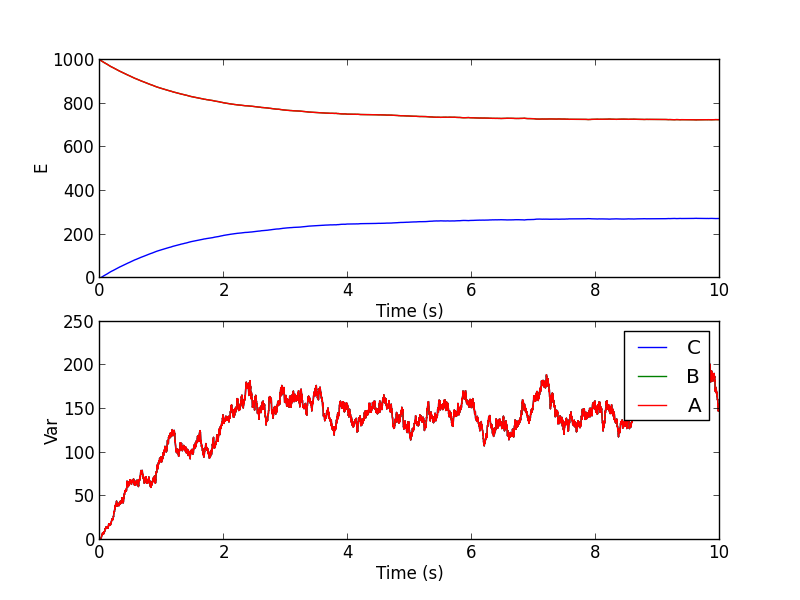
\includegraphics[width=0.75\textwidth]{Figures/BimolSpeciesTrace.png}
  \caption{Average (top) and Variance (bottom) of  the three species over 50 replicates for the reversible bimolecular reaction.} \label{fig:bst}
\end{figure}

\begin{figure}[h!]
  \centering
      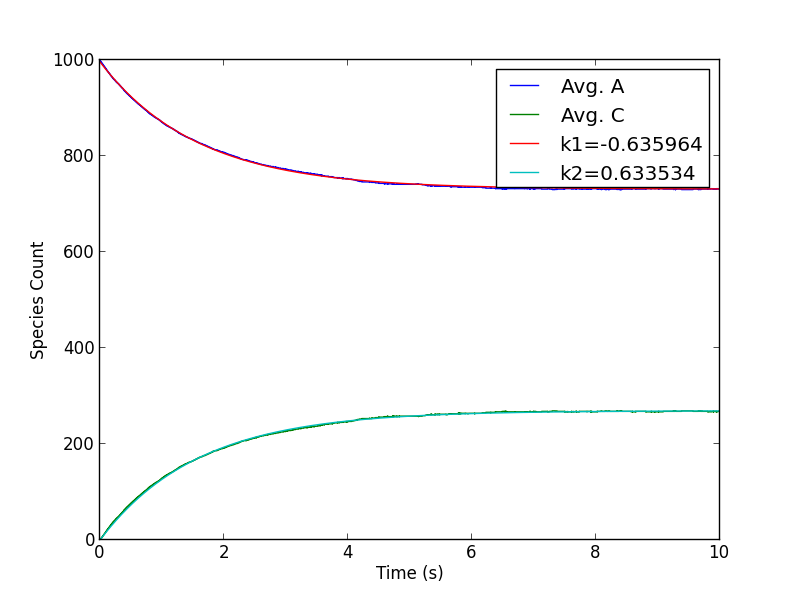
\includegraphics[width=0.75\textwidth]{Figures/BimolSpeciesFit.png}
  \caption{The same figure as before, except with fits to the rates performed in Python.} \label{fig:bsf}
\end{figure}

\begin{figure}[h!]
  \centering
      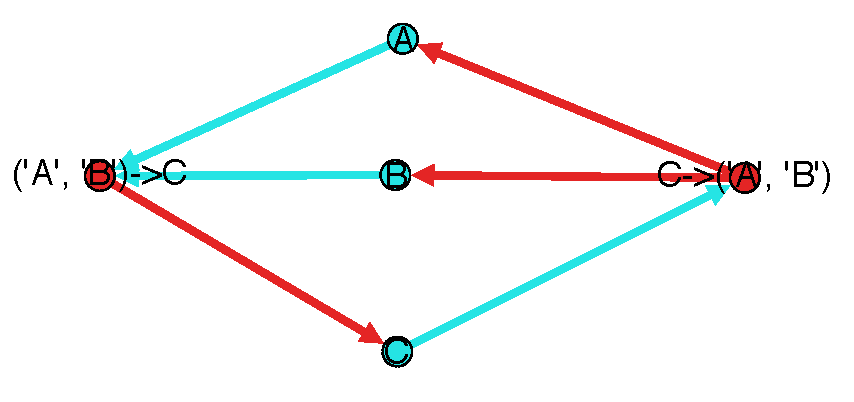
\includegraphics[width=0.75\textwidth]{Figures/RxnGraph.pdf}
  \caption{The graph of the simple bimolecular reaction.  Nodes in cyan are reacting species and red are reactions.  Direction of the arrows indicate flow of reactants.} \label{fig:graph}
\end{figure}


%%%%%%%%%%%
%Section: Difficulty%
%%%%%%%%%%%
\section{In case of difficulty}
If you experience problems when building the software, email the Lattice Microbes User List:\\ \url{latticemicrobes-users@lists.illinois.edu}.

Also, consider joining the Lattice Microbes User List by visiting: \\ \url{https://lists.illinois.edu/lists/info/latticemicrobes-users}


